% mnras_template.tex 
%
% LaTeX template for creating an MNRAS paper
%
% v3.0 released 14 May 2015
% (version numbers match those of mnras.cls)
%
% Copyright (C) Royal Astronomical Society 2015
% Authors:
% Keith T. Smith (Royal Astronomical Society)

% Change log
%
% v3.0 May 2015
%    Renamed to match the new package name
%    Version number matches mnras.cls
%    A few minor tweaks to wording
% v1.0 September 2013
%    Beta testing only - never publicly released
%    First version: a simple (ish) template for creating an MNRAS paper

%%%%%%%%%%%%%%%%%%%%%%%%%%%%%%%%%%%%%%%%%%%%%%%%%%
% Basic setup. Most papers should leave these options alone.
\documentclass[fleqn,usenatbib]{mnras}

% MNRAS is set in Times font. If you don't have this installed (most LaTeX
% installations will be fine) or prefer the old Computer Modern fonts, comment
% out the following line
\usepackage{newtxtext,newtxmath}
% Depending on your LaTeX fonts installation, you might get better results with one of these:
%\usepackage{mathptmx}
%\usepackage{txfonts}

% Use vector fonts, so it zooms properly in on-screen viewing software
% Don't change these lines unless you know what you are doing
\usepackage[T1]{fontenc}

% Allow "Thomas van Noord" and "Simon de Laguarde" and alike to be sorted by "N" and "L" etc. in the bibliography.
% Write the name in the bibliography as "\VAN{Noord}{Van}{van} Noord, Thomas"
\DeclareRobustCommand{\VAN}[3]{#2}
\let\VANthebibliography\thebibliography
\def\thebibliography{\DeclareRobustCommand{\VAN}[3]{##3}\VANthebibliography}


%%%%% AUTHORS - PLACE YOUR OWN PACKAGES HERE %%%%%

% Only include extra packages if you really need them. Common packages are:
\usepackage{graphicx}	% Including figure files
\usepackage{amsmath}	% Advanced maths commands
% \usepackage{amssymb}	% Extra maths symbols
\graphicspath{{../figures/}}

%%%%%%%%%%%%%%%%%%%%%%%%%%%%%%%%%%%%%%%%%%%%%%%%%%

%%%%% AUTHORS - PLACE YOUR OWN COMMANDS HERE %%%%%
\defcitealias{cristallo+11}{C11}
\defcitealias{cristallo+15}{C15}
\defcitealias{ventura+13}{V13}

\newcommand{\cristallo}{\citetalias{cristallo+11}+\citetalias{cristallo+15}}

% Please keep new commands to a minimum, and use \newcommand not \def to avoid
% overwriting existing commands. Example:
% \newcommand{\pcm}{\,cm$^{-2}$}	% per cm-squared
\newcommand{\VICE}{\texttt{VICE}}

%%%%%%%%%%%%%%%%%%%%%%%%%%%%%%%%%%%%%%%%%%%%%%%%%%

%%%%%%%%%%%%%%%%%%% TITLE PAGE %%%%%%%%%%%%%%%%%%%

% Title of the paper, and the short title which is used in the headers.
% Keep the title short and informative.
\title[Constraining carbon yields]{The galactic chemical evolution of carbon: Constraining stellar nucleosynthesis}

% The list of authors, and the short list which is used in the headers.
% If you need two or more lines of authors, add an extra line using \newauthor
\author[D. A. Boyea et al.]{
Daniel A. Boyea,$^{1}$\
et al.
% James W. Johnson,$^{1}$
% David Weinberg
% Jack Roberts
% Jennifer Johnson
% ?
\\
% List of institutions
$^{1}$Department of Astronomy, The Ohio State University\\
$^{2}$Department, Institution, Street Address, City Postal Code, Country\\
$^{3}$Another Department, Different Institution, Street Address, City Postal Code, Country
}

% These dates will be filled out by the publisher
\date{Accepted XXX. Received YYY; in original form ZZZ}

% Enter the current year, for the copyright statements etc.
\pubyear{2023}

% Don't change these lines
\begin{document}
\label{firstpage}
\pagerange{\pageref{firstpage}--\pageref{lastpage}}
\maketitle

% Abstract of the paper
\begin{abstract}
Stellar evolution models provide highly uncertain predictions for elemental yields due to our limited understanding of stellar physics. In this paper, we aim to estimate the nucleosynthetic yields of carbon using galactic chemical evolution models. 

We find that the AGB stars make up a fraction $0.20_{-20}^{+80}$ of total carbon production at late times. 
\end{abstract}

% Select between one and six entries from the list of approved keywords.
% Don't make up new ones.
\begin{keywords}
Need to find some...
\end{keywords}

%%%%%%%%%%%%%%%%%%%%%%%%%%%%%%%%%%%%%%%%%%%%%%%%%%

%%%%%%%%%%%%%%%%% BODY OF PAPER %%%%%%%%%%%%%%%%%%

\section{Introduction}

A fundamental question of Galactic Chemical Evolution (GCE) is understanding the physical processes which make each element. Stellar evolution models can be used to predict how much of each element stars with a variety of physical properties produce. However, these models are rife with uncertainties, limited by our understanding of critical physical processes such as nuclear reaction rates, convection, opacity, and mass loss (CITE, e.g. stellar physics reviews). 

Carbon and nitrogen are the only lighter elements produced significantly by low mass stars, so*****, reasons WHY this study. 

Asymptotic Giant Branch (AGB) stars are known to be importaint (cite) from stellar model predictions, previous GCE, and evidence from abundance patterns. (are there detections in PN?)

CCSNe are also important (.... SN reminant measurments)

We also know that there is evidence for non-monatonic carbon yield patterns. 
pattern where carbon is more readily produced by both high metallicity and very low metallicity stars (CEMPS, early GCE results), but our picture.

Additionally, stellar models are computationally expensive, even in one dimension, so while there are grids of predictions, these are not always fine enough to make accurate chemical evolution models. 

Previous models (CIte). We use \VICE (CITE) to create multi-zone models of GCE enabling us to account for the effects of migration on our predicted yields. 

\citet{prantzos+18}
\citep{WAF17}
\citep{james+21}
\citep{fiorenzo+21}


\citep[e.g.][]{james+22}

Carbon abundances are strongly affected by CNO cycle processing in stars. The CNO cycle is one of two series of nuclear reactions( $^{12}$C(p, $\gamma$)$^{13}$N($\beta^+ \nu_e$)$^{14}$N(p, $\gamma$)$^{15}$O($\beta^+\nu_e$)$^{15}$N(p,$\alpha$)$^{12}$C

Because the $^{14}$N(p, $\alpha$) proton capture is the slowest component of the CNO cycle ****, the CNO cycle, to first order, converts all $^{12}$C into $^{14}N$. 

One challenge of measuring abundances of carbon in star is that when a star becomes a RGB star, material from the CNO-processed core. Since this core-processed material is now carbon depleted and nitrogen enhanced, measurments of this star's atmosphere will no longer reflect the birth abundances of the star.

In Figure \ref{fig:sum} we present a sample of APOGEE subgiants. These subgiants were chosen based on their location in the HR diagram based on criteria in \citet{jack_subgiant} replicated in Appendix \ref{sec:jack}. Because subgiants have not undergone FDU, their surface abundances are an accurate reflection of the birth abundances (CITATION).  




\begin{figure*}
    \centering
    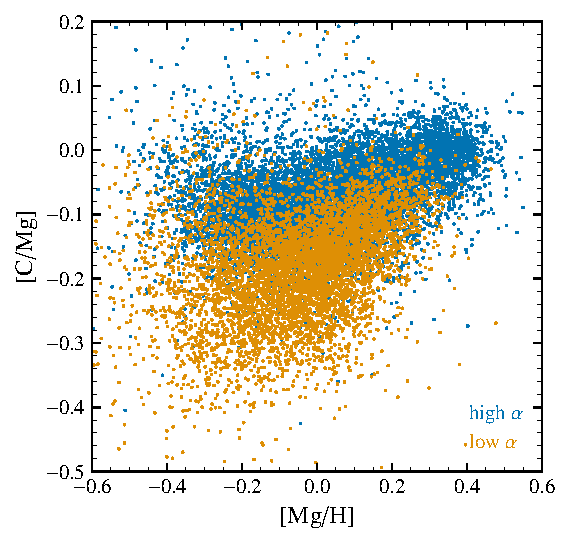
\includegraphics[]{subgiants_mgh.pdf}
    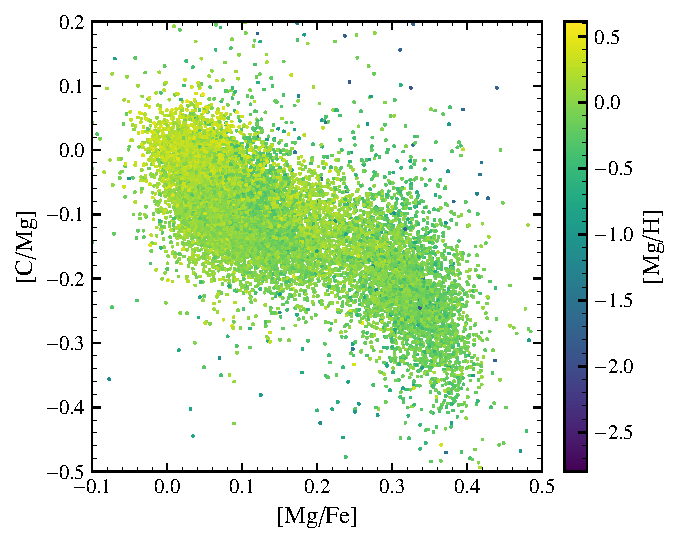
\includegraphics[]{subgiants_mgfe.pdf}
    \caption{Chemical abundance relationships of our sample of APOGEE subgiants (see Jack et al. 2023). Left panel shows }
    \label{fig:sum}
\end{figure*}
\section{Nucleosynthesis}

Galactic chemical evolution are fundamentally intertwined with our understanding of stellar nucleosynthesis. In this paper, we are concerned with three major nucleosynthetic pathways: AGB stars, CCSNe, and Supernovae type Ia. While only AGB stars and CCSNe are producers of carbon, SNeIa Fe can be used to compare with the AGB delayed carbon component. 

\VICE allows us to explore the nucleosynthesis of various models, as it includes AGB tables for C11, et.c
    
We discuss carbon nucleosythesis in more detail in the next two sections. We assume that the only dominant sources of carbon are from AGB stars and CCSNe/massive star winds. ***JUSTIFY***. Below  is a brief overview of our  nucleosythetic assumptions of other elements.

Let $y_{\rm X}^{\rm proc}(M, Z)$ be the fractional yield of element X by a process proc for stars of a mass $M$ (in solar masses) and at metallicity $Z$ defined as: 
\begin{equation}
    y_{\rm X} = \frac{M_{\rm X,\ ej} - M_{\rm X,\ birth}}{M}   
\end{equation}

Where $M_{\rm X,\ ej}$ and $M_{\rm X,\ birth}$ are the mass of element X ejected and initially present in the star. 
We define the IMF-integrated yield of X with: 
\begin{equation}
Y_{\rm X}^{\rm proc}(Z) = \int_{M_{\rm min}}^{M_{\rm max}} y_{\rm X}^{\rm proc}(M, Z)\ \Phi(M)  \ dM
\end{equation}
Where $\Phi(M) = \frac{dN}{dM}/ \int_{M_{\rm min}}^{M_{\rm max}} \frac{dN}{dM}\ dM$ is the normalized IMF, $M_{\rm min}$ and $M_{\rm max}$ are the minimum and maximum mass of stars, which we take to be $0.08 M_{\sun}$ and $100 M_{\sun}$ respectively; and $\frac{dN}{dM}$ is the initial mass function, the frequency of stars born between $M$ and $M+dM$.

There are two $\alpha$-elements we care about: Mg and O. Stellar observations of magnesium are more reliable but oxygen abundances are easier to measure in HII regions. We assume that both Mg and O are produced entirely in CCSNe with constant, metallicity-independent yields. Thus $\text{[Mg/H]} = \text{[O/H]} = [\alpha/\text{H}]$ in our models

\begin{itemize}
    \item observational validation
\end{itemize}
For carbon, the dominant producer is from massive stars which eject carbon fused in their cores during CCSNe. 

Taken from J21 and J22, we make the following yield assumptions:
\begin{itemize}
    \item $Y_\text{O}^\text{CC} = 0.015$
    \item $Y_\text{O}^\text{Ia} = 0$
    \item $Y_\text{Fe}^\text{Ia} = 0.00214?$
    \item $Y_\text{Fe}^\text{CC} = 0.0012$
    \item $Y_\text{N}^\text{CC} = 0.00036$
    \item $y_\text{N}^\text{AGB}(M, Z) = 9\times 10^{-4} M \left(\frac{Z}{Z_\odot}\right)$
\end{itemize}
Also following J21/J22, we take the SNeIa Delay Time distribution to be a $t^{-1.1}$ law based on
the observations by \citet{maoz+12}.

We leave consistent throughout the paper. While different CCSNe models predict different absolute values for $y_\text{O}^\text{CC}$, they also predict that the yield is metallicity-independent within the uncertainties of the model. 





\subsection{Asymptotic giant branch carbon}

An AGB star is a low mass ($\lesssim 8 M_{\sun}$) star during the final phases of evolution. The star has already completed Hydrogen core burning, Hydrogen shell burning during the red giant branch phase, and Helium core burning. So, the structure consists of an inert core of carbon and oxygen surrounded by a Helium burning shell and a Hydrogen burning shell. The double shell burning leads to thermal instabilities which drive off the outer layers of the star in a series of violent pulsations, ejecting the envelope and leaving behind a C/O white dwarf. 

In an AGB star, TDU and HBB are two major processes involved in carbon production and destruction. TDU occurs during thermal pulsations, where the convective layer of the star passes into the inner layers with He-burning products which mixes in C and O into the envelope. In contrast, HBB may happen if the base of the convective envelope reaches about 50MK, initiating the CNO cycle, converting most C12 into N14. 

The differences in yields between AGB models depend on the mass loss rate, treatment of convection, and nuclear reaction rates. 

In this work, we explore four different sets of AGB star yields representative of the variety of options which also provide reasonably well sampled grids in metallicity and mass necessary for chemical evolution studies.
\begin{itemize}
    \item \citetalias{cristallo+11}
    \item \cristallo
    \item \cite[C11][Hi]{cristallo+11}: \citet{cristallo+11}
    \item K10: \citet{karakas10}
    \item V13: \citet{ventura+13}
    \item K16: \citet{KL16}
\end{itemize}
Unless otherwise noted, C11 is the model we choose as our fiducial AGB yield. 

Figure \ref{fig:y_agb} compares the net fractional AGB carbon yield, $m_\text{C}^\text{AGB}(M, Z)$ for each AGB model we consider. Note that the yields may be negative when the birth abundance is higher than the carbon abundance of the material ejected back to the ISM. 

Most models agree on the qualitative shape of the net fractional AGB carbon yield. The stars with the highest fractional carbon yields are between 2 to 4 solar masses, depending on the metallicity and model. Both lower and higher mass stars produce less carbon, and high mass stars may even destroy carbon at high metallicity due to highly efficient HBB. And all models agree that the carbon yield generally decreases with metallicity. 


Metallicity dependence:
V13 is the only model that stands out, showing a non-monotonic metallicity dependence, however this effect is only for models with [M/H]$\leq -1$. Otherwise the major differences between the models are the precise amount of carbon and the slope of the metallicity dependence. For example, the three models C11, K10, and K16 predict $y_\text{C}^\text{AGB}$ to be between 0.006 and 0.008 at solar metallicity, but C11 has a much shallower metallicity dependence than the K10 and K16 models. And at solar, V13 predicts a value at around 0.004 so the models are all within about a factor of 2. 

Another difference is the speed at which equilibrium is reached. K10 and K16 weight carbon production more heavily towards massive stars resulting in a faster time to equilibrium, whereas the C11 and V13 models predict a slightly longer timescale with order 1Gyr, but little to no carbon is produced more than 2Gyr after a star formation event. This is in contrast to iron which is still produced by SNeIa up to 10Gyr after a star formation event. 

\begin{figure*}
    \centering
 	    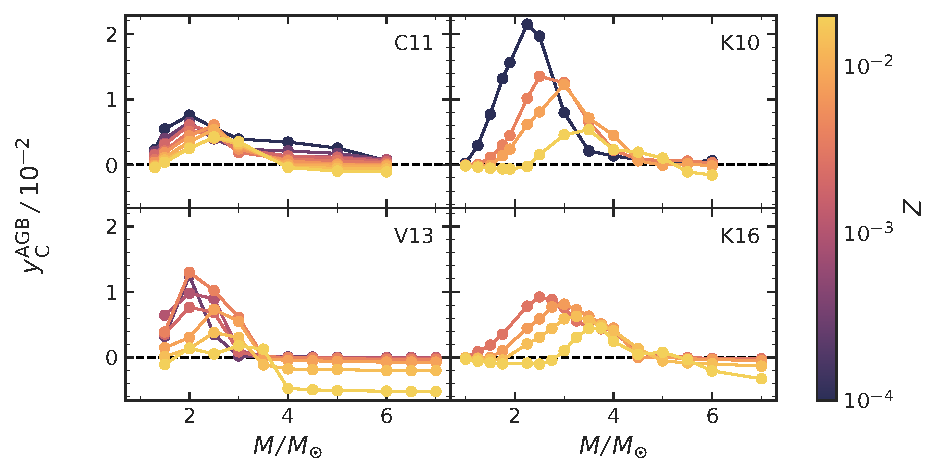
\includegraphics[scale=1]{agb_yields.pdf}\\

    \caption{The net fraction carbon yield ($M_\text{C}$, the amount of carbon produced by the star divided by $M$) plotted as a function of mass, $M$. Lighter colors represent higher values of metalicity ([M/H]). Each panel represents a different AGB model. K10 reports stars at MoverH -3, -2, etc. I can reproduce C11 and K10 but not other V13 and KL16 :(((}

    \label{fig:y_agb}
\end{figure*}

\begin{figure*}
    \centering
    
    \includegraphics[scale=1]{y_agb_vs_z-1.pdf}
    \includegraphics[scale=1]{y_agb_vs_t-1.pdf}

    \caption{On the left, we plot the IMF weighted net fractional carbon yields of each AGB model as a function of metalicity.The right panel plots the normalized net carbon AGB yield as a function of time for a population of stars born at the same time at solar metallicity. We note that for the right panel, the minimum of the DTD for V13 is }

\end{figure*}

\subsection{CCSNe carbon}

While there are many stellar models providing predictions of CCSNe yields, the results of these models are highly uncertain due to the many stellar modeling uncertainties. 

We summarise many of the predictions of stellar models in Figure \ref{fig:y_cc}. Pink squares
represent \citep{NKT13}, etc. etc.
\citep{LC18}
\citep{sukhbold+16}
\citep{WW95}

On the right, we plot the expected CCSNe abundance ratio of each model as a function of metallicity, defining
\begin{equation}
    {\rm [C/O]^{CC}} = \log_{10}\left( \frac{y_{\rm C}^{\rm CC}}{y_{\rm O}^{\rm CC}}\right) - \log_{10} \left( \frac{Z_{C, \sun }}{Z_{O, \sun }} \right)
\end{equation}
Notice how even these ratios 
\begin{figure*}
    \includegraphics[scale=0.9]{y_c_cc-2.pdf}
    \includegraphics[scale=0.9]{y_co_cc.pdf}
    \caption{The fist plot shows IMF-weighted net fractional CCSNe yield of carbon, $y_C^{cc}$ against metalicity, [M/H], for different studies. The right plot instead shows [C/O]$^\text{CC}$, the logarithm of the abundance ratio of carbon to oxygen if CCSNe were the only carbon source, also as a function of metallicity for the same set of studies. The black line represents the carbon yield of the fiducial model, $y_C^{CC} = 0.004? (Z/Z_{\sun})^{0.3}$, and becomes dashed over regions where we have not tested our model. }
    \label{fig:y_cc}
\end{figure*}

    \begin{itemize}
        \item Wide range in predictions, exacerbated to 1 dex range when including variance in oxygen predictions
        \item (explain) most models have a near-metallicity independent oxygen yield, so we choose the fiducial value of 0.015 despite varience in $y_O^{cc}$
        \item The fiducial value, where we choose the carbon yield from Sukhbold+16, may be above most predictions of carbon yields but is within the range of yield ratios
        \item the fiducial value would reach an equilibrium carbon yield of -0.1 without AGB stars
        \item Rotation in LC18 appears to increase metallicity dependence of carbon production (read this paper more carefully)
        \item NKT and LC agree in positive metallicity depenent yields
    \end{itemize}
    

\section{The Multizone Model}

To simulate the chemical evolution of a Milky way like galaxy, we use the Versitile Integrator for
Chemical Evolution (\VICE\footnote{\VICE~is available at \url{https://github.com/giganano/VICE}}) published in \citet{james+21} and also briefly described in
\citet{james+22}. 
As a multi-zone model, the galaxy is divided into 200 rings of 0.1kpc, each with separate gas supplies with outflow and inflow rates.


\VICE\ accounts for radial migration by using the results of the \texttt{h277} hydrodynamical simulation. Each VICE SSP is matched to a random nearby star particle \textit{analogue} in \texttt{H277}. VICE approximates the migration of this particle by using a $\sqrt{\text{time}}$-diffusion approximation where the change in galactic radius of a star, $\Delta R$, is $\Delta R \propto \sqrt{\text{t}}$. 
VICE does not account for radial gas flows. 

Other approaches have used dynamical arguments to implement their stellar mirgrations. We note that our approach does not introduce more free parameters which may bias conclusions. However, we only consider one dynamic history, and it is still unknown how variations in the dynamic history of a galaxy impact its chemical evolution.


We initially assume an "inside-out" SFH where the star formation rate peaks in the early evolution of the galaxy and is higher closer to the galactic center. The star formation rate, $\Sigma_\star$, for our fiducial model is parameterized by
\begin{equation}
    \dot{\Sigma}_\star \propto \left(1-e^{-t/\tau_{\rm rise}}\right) e^{-t/\tau_{\rm sfh}}
\end{equation}
where $\tau_\text{rise}=2$Gyr is the
and $\tau_{sfh}$ is the rate of decline of the star formation rate, which is based on *****.

We also explore a "lateburst" model which is parameterized with a normal distribution multiplying our fiducial "inside-out" SFH as
\begin{equation}
    \dot{\Sigma}_{\rm lateburst} \propto \dot{\Sigma}_{\rm insideout} \left(1 + A e^{-(t-\tau_{\rm burst})^2/2\sigma^2_{\rm burst}} \right)
\end{equation}

$A=1.5$ represents the amplitude of the birth, $\tau_\text{burst}=10.8$Gyr is the time where the burst is strongest, and $\sigma_\text{burst}=1$Gyr is the width of the burst. We do explore the effects of variations of this parameterization in section ****.


VICE normalizes the total mass of star formation against observations from ******.
The gas inflow is calculated based on our star formation parameterization by using a schmit law 
\begin{equation}
    dM_g \propto \dot{\Sigma}^{1/n}
\end{equation}
where we take $n$ to be ****

Salpeter IMF.

\subsection{Yield Parameterization}
  Because of the large uncertainties in CCSNe carbon yields, we choose to explore an analytic expression of the yield enabling us to easily explore how variations of CCSNe carbon yields affect abundance tracks. We find that a powerlaw yield with a metallicity-dependent constant minimum is able to match the observations well while remaining a simple parameterization (see below). Our expression is:
    \begin{equation}
   y_\text{C}^\text{CC}(Z) =  \alpha\ Z^\beta y_\text{O}^\text{CC} + y_\text{C, 0}^\text{CC}
    \end{equation}
   	Where we estimate $\alpha = 0.02$ and $\beta = 0.25$ (See Section \ref{equilibrium} ). Our second model uses $\alpha = 0.44$ and $\beta = 0.63$ with K16 yields and reduced $\eta \rightarrow 1/2 \eta$ 
    
    As an overall scaling of yields does not significantly affect our models, we choose to fix the total equilibrium value of the total carbon yield at solar at $Y_{\text{C},\ \sun} = 0.005$, and then scale the yields relative to this value. 

\section{Multizone model results}


\subsection{Data Selection}

We use data from APOGEE DR17 processed with APOSCAP. Since subgiant stars have yet to experience FDU, their atmospheric carbon and nitrogen abundances are still reflective of their birth abundances and do not need mixing corrections. 

To select for subgiants, we use the following cut in $\log g$ and $T_{\rm eff}$ which selects stars at the base of the red giant turnoff (FIGURE and \cite{jack_subgiant})

Because the star formation history is left in a simple inside-out form, this multizone model does not reproduce the high-$\alpha$ sequence, therefore we make the following cut to the V21 data to remove the high alpha sequence.

\begin{equation}
\begin{cases}
\text{[Mg/Fe]} >0.12-0.13\text{[Fe/H]}, & \text{[Fe/H]}<0\\
\text{[Mg/Fe]} >0.12, & \text{[Fe/H]}>0\\
\end{cases}
\end{equation}


See Appendix \ref{sec:jack} for further discussion of our sample and comparison to FIORENZO.


\subsection{The Evolution of carbon across the galaxy and through time}

The GCE of carbon is complicated by metallicity dependencies and delayed contributions. 

We note the following features of our model:

\begin{enumerate}
    \item Carbon comes predominantly ($\sim80\%$) from CCSNe but the rest is from AGB stars
    \item The CCSNe carbon production is more efficient at higher metallicities
    \item AGB stars produce less carbon at higher metallicities.
\end{enumerate}


The combination of these features leads to an evolution that proceeds as follows
\begin{enumerate}
    \item Initially, CCSNe dominate production before AGB stars can contribute their enrichment, but because CCSNe is highly metalliticy dependent, the C/$\alpha$ ratio increases with time.
    \item AGB stars begin contributing their carbon, increasing the $C/\alpha$ ratio more steeply as the gas begins to reach its equilibrium metallicity
    \item When $Z$ reaches equilibrium, the $C/\alpha$ ratio stops increasing or may even decline, as AGB stars formed at higher metallicities reduce the net carbon yields.
\end{enumerate}

We plot time evolution tracks in Figure \ref{fig:c_evo} for $[C/\alpha]-[\alpha/H]$ and $[C/\alpha]-[Fe/H]$ for our fiducial model. Each colored track corresponds to a different galactic radius and 1Gyr time steps are marked with crosses on the lines. 

Comparing [C/$\alpha$] against [Fe/H] enables us to see late time evolution of carbon more clearly. Because [Fe/H] takes longer to reach equilibrium as half of iron production comes from type-Ia supernovae, the late time evolution is not clustered as tightly horizontally as for [$\alpha$/H].

This is even more evident in the lower part of Figure \ref{fig:c_evo}, where we instead plot snapshots of the galactic radial trend at different times for our model. While the [C/$\alpha$]-[$\alpha$/H] trend reaches almost equilibrium at 5Gyr, the [C/$\alpha$]-[$\alpha$/Fe] trend continues to evolve even until the present day, exposing the effect of the delayed contribution from AGB stars on the evolutionary history.

\begin{figure*}
\label{fig:c_evo}
\includegraphics{evo_tracks-9.pdf}
\includegraphics{evo_slices-2.pdf}
\caption{The top set of panes show the time evolution of the gas phase of our fiducial model, plotted as tracks through [C/O]-[O/H] and [C/O]-[O/Fe] where each colored line corresponds to the evolution at that galactic radius. 
The bottom set instead shows the galaxies gas-phase [C/O]-[O/H] and [C/O]-[O/Fe] trend at 5 different time slices. 
}
\end{figure*}




\subsection{Effects of AGB Yields}
\begin{figure*}
\includegraphics[scale=0.6]{oob_agb-1.pdf}

\caption{Abundance tracks for 4 different choices of AGB models. Each panel has different abundance ratios on the axis but is otherwise the same. The black points are Jack Roberts selection of APOGEE subgiants. Each model is plotted as a line representing the mean stellar abundance in each bin on x.}
\label{fig:stars_abundances}
\end{figure*}


How much does the choice of AGB model affect chemical evolution? 
Short description of effects of AGB model choices, and how we can rule out models like V21.  Maybe point to appendex B?


Our next exploration is to adjust the relative fraction of AGB star yields. To do this, we hold the total carbon yield at solar metallicity fixed, so for a desired AGB fraction (assuming equilibrium), 


\begin{equation}
    \alpha_{AGB} = f_{agb} \frac{y_{desired}}{y_0^{agb}}
\end{equation}
\begin{equation}
    \alpha_{CC} = (1 - f_{agb}) \frac{y_{desired}}{y_0^{cc}}
\end{equation}




\subsection{Star Formation History}

We do run models with an alternate "lateburst" stars formation history.

equation of lateburst

However, we find that the star formation history has a negligable effect on the shape of the mean track. More drastic changes in SFH could explain the high alpha/low alpha seperation but we leave further exploration of SFH to future work. 


% \begin{figure*}
% \includegraphics[width=1.5\columnwidth]{cooh_lateburst.pdf}
% \caption{Same as Fig. \ref{fig:stars_abundances} but with different model choices.}
% \end{figure*}



\begin{figure*}
\includegraphics[scale=0.6]{beta-1.pdf}
\includegraphics[scale=0.6]{f_agb-1.pdf}

\caption{Similar to \ref{fig:stars_abundances} except the top plot shows the fiducial model with lower and higher values of $\beta$, the C-CCSNe metallicity dependence. The bottom plot is the same except shows varying AGB fractions.}
\end{figure*}

\begin{figure*}
\includegraphics[scale=0.6]{lateburst_eta-1.pdf}

\caption{Same as Figure \ref{fig:stars_abundances} but comparing the fiducial model to the reduced outlow model and a lateburst model. (okay, need to totally change approach...)}
\end{figure*}

\subsection{Adjusted CCSNe Yields}

\begin{figure}
    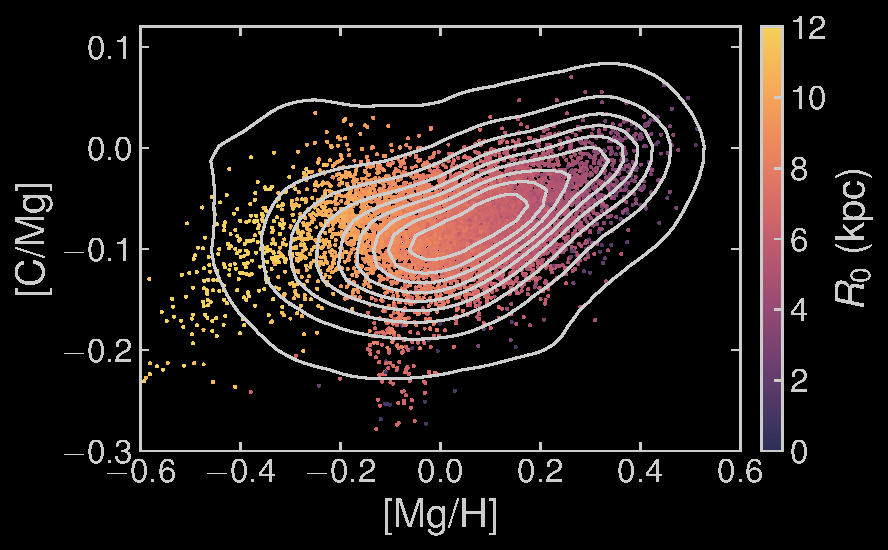
\includegraphics[scale=0.6]{cooh_scatter.pdf}
    \caption{The simulated stars of our model at present day plotted on [C/O]-[O/H] and colored such that lighter colors represent stars born at greater galactric radii.}
\end{figure}

\begin{figure}
    \centering
    \includegraphics[scale=0.6]{cnoh.pdf}
    \caption{Caption}
    \label{fig:cnofe}
\end{figure}


\begin{figure*}
\centering
\includegraphics[]{summary-2.pdf}
\caption{Present-day gas phase tracks of the fiducial model in [C/O]-[O/H] space. M101 is valid comparison to MW ...(van Dokkum et al. 2014)}
\label{fig:gas_phase}
\end{figure*}
\subsection{The AGB Fraction }
One potential tension with data is our models predict a low value for the AGB fraction of stars. 

Our model with Z-dependent CCSNe yields has $f_\text{agb} = 0.05$ which implies that CCSNe overwhelms AGB production and there should not be a seperation between low and high alpha sequences. However, V21 observes a significant seperation implying a more substantial delayed-time source. 

Even changing the AGB model does not affect the conclusion significantly. 

An alternate solution is to reduce the outflows and core collapse yields similarly, consistent with a model where more large stars collapse directly into black holes. This leaves the $y_\text{C}^\text{CC}/y_\text{O}^\text{CC}$ ratio unchanged, but because $y_\text{C}^\text{CC}$ is unchanged, the relative size of the AGB contribution is larger. 


Increasing the relative AGB production lowers the magnitude of  $y_\text{C}^\text{CC}/y_\text{O}^\text{CC}$, but the metallicity dependence of the ratio must increase to compensate for the inverse metallicity dependence of AGB carbon yields. 

We find that we can adjust both the outflows and scale down the yields if we change our model for $y_\text{C}^\text{CC}/y_\text{O}^\text{CC}$. For example, reducing outflows and CCSNe yields by a factor of two requires the modified parameters
$\alpha = 0.033$ and $\beta = 0.625$, which results in a slightly lower value at solar but nearly a doubling of the metallicity dependence.

These models are indistinguishable in the [C/O]-[O/H] plane from our adjusted CCSNe model, so future work investigating the SFH and carbon isotopic ratios in more depth may be able to provide more insight. In the next section, we develop the analytic tools to explore this problem in more depth. 

\subsection{Outflows}
A common degeneracy in chemical evolution models is the yield-outflow degeneracy. An increase in stellar yields has a near-identical effect as a decrease in outflows. However, reducing the outflows reduces the evolution timescale of the system. 

The theoretical motivation for decreasing outflows is due to the uncertainty in the explodability landscape---if less massive stars explode, then both the yields and outflows will be reduced by some factor. So, when we explore reduced outflow models, we consider models where both the outflows and yields are reduced by approximately the same factor, to leave the equilibrium abundances of a pure CCSNe unchanged. 

The effect of reducing outflows is then increasing the relative contributions of non-CCSNe processes. For carbon, this increases the AGB fraction.

We have found that the [C/O]-[O/Fe] relationship may provide insight into this issue. [O/Fe] is a tracer of the relative contributions of CCSNe and delayed-time sources in chemical evolution. So, the appearance of a slope in [O/Fe] implies that there is a substantial delay-time process in carbon evolution. 
The metallicity-dependence of carbon yields complicates this picture because younger stars have higher [O/Fe] as the SNeIa contributions take up to 10Gyr, so metal-poor young stars will naturally have lower [C/O], agreeing with the slope observed in [C/O]-[O/Fe]. However, a pure CCSNe carbon model cannot reproduce the slope accurately as  



\subsection{Comparison to HII Region Observations}
In Figure \ref{fig:gas_phase}, we plot our two favorite models against HII-region measured carbon abundances from **********

Our model appears to be broadly consistant with the gas phase data, however these imply if anything that the slope should be increased. 

Are HII regions a good approximation?

Short discussion of measurment challenges in extragalactic galaxies, how other galaxies and dwarf SFH may come into play, why this relation is notecably steeper.

\section{The Equilibrium Approximation}\label{equilibrium}
If we assume that the median track is an equilibrium phenomenon, we can calculate the total carbon to oxygen yield ratio. Additionally, assuming an AGB yield set enables us to predict the CCSNe carbon yield.  
We begin with the model, which underlies the multizone simulations, that the change in mass of an element is a sum of production, outflows, recycling, and mass left in reminants. We write this as
\begin{equation}
M_\text{C} = y_\text{C} \dot{M}_\star - (1 + \eta - r) Z_\text{C} \dot{M}_\star
\end{equation}

In the case that carbon
\begin{equation}
Z_c^{eq}(R) = \frac{y_c^{cc} + \langle y_c^{agb} \rangle }{1 + \eta(R) - r - \tau_\star / \tau_{sfh}}
\end{equation}Where
\begin{equation}
\langle y_c^{agb} \rangle = \frac{\int_0^T y_c^{agb}(M, Z) \dot{M}_\star(T - t) \frac{dN}{dM} \frac{dM}{dt} dt  }{ \dot{M}_\star \int_0^T \frac{dN}{dM} \frac{dM}{dt} dt}
\end{equation}

Likewise for oxygen:
\begin{equation}
Z_O^{eq}(R) = \frac{y_O^{cc}}{1 + \eta(R) - r - \tau_\star / \tau_{sfh}}
\end{equation}

However, for the yield ratio, the denominator cancles with that of oxygen, so the ratio is fixed.
\begin{equation}
\frac{Z_c^{eq}}{Z_o^{eq}} = \frac{y_c^{cc} + \langle y_c^{agb} \rangle }{y_o^{cc}}
\end{equation}

For this analysis, we let $y_c^{agb}$ represent the default AGB yields from a given yield set, but add a process factor $\alpha_{agb}$ which multaplicatively increases the AGB fraction. See Table \ref{tab:alpha_agb}.

\begin{equation}
    y_{\rm C}^{\rm CC} \rightarrow \alpha_{agb}  y_{\rm C}^{\rm CC}
\end{equation}

With these definitions, we can calculate the core collapse yields of carbon as a function of metallicity:
\begin{equation}
    y_\text{C}^\text{CC} =  y_\text{O}^\text{CC} \frac{Z_\text{C,eq}}{Z_\text{O,eq}} - \alpha_{agb} \langle y_c^{agb} \rangle
\end{equation}

Rewriting in terms of the observed abundance ratio and dividing by $y_\text{O}^\text{CC}$. So, given the outflows or CCSNe oxygen yields, the carbon AGB yield, and the [C/O]-[O/H] mean abundance track, we can estimate the CCSNe carbon yield. Written as a relative yield:
\begin{equation}
    \frac{y_\text{C}^\text{CC}}{y_\text{O}^\text{CC}} = \frac{Z_{C, \sun}}{Z_{O, \sun}} 10^{[C/O]} - \frac{\alpha_{agb} \langle y_c^{agb} \rangle}{ y_\text{O}^\text{CC}}
\end{equation}

This equation corroberates what we have explored earlier in the paper, and provides our analytic estimates of the CCSNe carbon yields. Since the AGB term is subtracted, a negative AGB Z-dependence will correspond to a positive CC Z-dependence. And as we reduce outflows, the AGB factor increases, steepening the required slope of the carbon yields. So, while the AGB yields may agree with eachother, the uncertainties in the oxygen CC yields and outflows leads to a substantial uncertainty in the AGB fraction.  

\begin{figure}
    \centering
    \includegraphics[scale=0.3]{analytic_y-4.pdf}
    \caption{Our reverse fitting method to determine total CCSNe contribution}
\end{figure}

% y_c^cc = (0.0148 +- 0.00016) Z^{0.154 +- 0.0053}
\begin{equation}
    y_C = (0.004 \pm 0.00002) + (0.008 \pm 0.0001) \text{[M/H]} 
\end{equation}

\subsection{Uncertainties}

We only perform this analysis on the C11/15 yields because the range of metallicities of the data (about [M/H] = -0.4, 0.4) only represents about 2 AGB models, relying heavily on our choice of extrapolation. C11/C15 have a finer model grid, allowing us to have 5 theoretical predicted points within this metallicity range, allowing us to be more certain of our conclusion. 

We do note that this analysis fails to take into account selection effects and biases in APOGEE, and a more robust determination of the carbon yield. 


This formulation is degenerate in $\varpi$ until we estimate a better AGB fraction. As the seperation between the low and high alpha sequences can be used to estimate the delayed time contribution to carbon, using the model to estimate this value relies heavaly on the details of the SFH in addition to the 
We do give an estimate of the CCSNe yields, however this is dependent on our choice of $\eta$. Other choices of $\eta$ vary the value significantly in both magnitude and slope (as AGB contributions increase, we need less CCSNe carbon, however the CCSNe carbon must have a higher metallicity dependence to replicate the V21 data). 


\section{Modeling extragalactic carbon trends}
Can we use our yield estimations and apply them to extragalactic sources successfully? 

Explain Berg+19,

Bursty SFH may not be needed to explain scatter as the C/O slope + differet evolutionary timescales is capable alone of reproducing this scatter.

While the extragalactic trend appears to be more steeply sloped than our models, this is because of ***e.g. mass-dependent outflow rates/differening SFH between galaxies. 


\section{Conclusions}

The last numbered section should briefly summarise what has been done, and describe
the final conclusions which the authors draw from their work.

\section*{Acknowledgements}

The Acknowledgements section is not numbered. Here you can thank helpful
colleagues, acknowledge funding agencies, telescopes and facilities used etc.
Try to keep it short.

Numpy, pandas, scipy, VICE, matplotlib
\cite{numpy, matplotlib}

\cite{OhioSupercomputerCenter1987}

%%%%%%%%%%%%%%%%%%%%%%%%%%%%%%%%%%%%%%%%%%%%%%%%%%
\section*{Data Availability}

 
The inclusion of a Data Availability Statement is a requirement for articles published in MNRAS. Data Availability Statements provide a standardised format for readers to understand the availability of data underlying the research results described in the article. The statement may refer to original data generated in the course of the study or to third-party data analysed in the article. The statement should describe and provide means of access, where possible, by linking to the data or providing the required accession numbers for the relevant databases or DOIs.




%%%%%%%%%%%%%%%%%%%% REFERENCES %%%%%%%%%%%%%%%%%%

% The best way to enter references is to use BibTeX:

\bibliographystyle{mnras}
\bibliography{main} % if your bibtex file is called example.bib


% Alternatively you could enter them by hand, like this:
% This method is tedious and prone to error if you have lots of references
%\begin{thebibliography}{99}
%\bibitem[\protect\citeauthoryear{Author}{2012}]{Author2012}
%Author A.~N., 2013, Journal of Improbable Astronomy, 1, 1
%\bibitem[\protect\citeauthoryear{Others}{2013}]{Others2013}
%Others S., 2012, Journal of Interesting Stuff, 17, 198
%\end{thebibliography}

%%%%%%%%%%%%%%%%%%%%%%%%%%%%%%%%%%%%%%%%%%%%%%%%%%

%%%%%%%%%%%%%%%%% APPENDICES %%%%%%%%%%%%%%%%%%%%%

\appendix

\section{Validating the APOGEE Subgiant Sample}\label{sec:jack}
Our APOGEE subgiant sample excludes stars marked with the following flags:
\begin{itemize}
\item \texttt{ancillary young embedded cluster}
\item \texttt{ancillary emission line star}
\item \texttt{MIR-deected candidate cluster member}
\item \texttt{selected as part of the EB program}
\item \texttt{selected as part of the young cluster study (in-SYNC)}
\item \texttt{W3/4/5 star forming complex}
\end{itemize}

To select stars only in the subgiant branch, we select stars in a polygon in $\log g$-$T_\text{eff}$ space described by the following cuts:
\begin{equation}
\begin{cases}
\log g \geq 3.5 \\
\log g \leq 0.004\ T_\text{eff} - 15.7 \\
\log g \leq 0.00070588\ T_\text{eff} + 0.358836 \\
\log g \leq -0.0015\ T_\text{eff} + 12.05 \\
\log g \geq 0.0012\ T_\text{eff} - 2.8 \\
\end{cases}
\end{equation}

Instead of excluding stars which have experienced FDU and thus modified carbon abundances as JACK's subgiant sample does, another approach to predict the birth abundances of carbon and nitrogen in stars is to model the predicted abundance effects of dredge up and then correct the measured abundances, as is done in V21. 

In the first panel, both V13 and the subgiant sample predict similar trends in [C/Mg]-[Mg/H] but there appears to be a systematic offset of about 0.2dex. Reproducing the trend is promising as V21's mixing corrections were metallicity-dependent so the uncorrected sample of APOGEE giants does not match the subgiant trend. 

The systematic offset could be explained by overpredicting the effects of FDU or other *** in V21's stellar evolution models??? or other subgiant physics???

In the second panel, agreement appears to be better. Both the MDF and the slope are nearly identical,
There is a slight deviation in slope between the models, and this could again be a systematic such as underestimation of **8some stellar effect**** at higher metallicities.

We compare both of **** in Figure \ref{fig:fiorenzo_jack}.


\begin{figure*}
    \centering
    \includegraphics[scale=0.5]{fiorenzo_vs_jack_c-1.pdf}
    \includegraphics[scale=0.5]{fiorenzo_vs_jack_n-1.pdf}
    \caption{A comparison of estimated stellar birth abundance trends from the subgiant sample and
        \citet{fiorenzo+21}
    }
    \label{fig:fiorenzo_jack}
\end{figure*}

\section{Effects of Alternate AGB Models}\label{sec:alt_agb}

\begin{table}
	\centering
	\caption{For each AGB yield set, our calculation of the effective SFH- and IMF-weighted carbon AGB yield, along with the multiplicative factor to reach an AGB contribution of 20.}
	\label{tab:alpha_agb}
	\begin{tabular}{lcr} % four columns, alignment for each
		\hline
		Study & $y_{\rm C, 0}^{\rm agb}$ & $\alpha_{\rm agb, 20}$\\
		\hline
		C11 & 0.000347 & 2.9\\
		K10 & 0.000585 & 1.7\\
		V13 & 0.000060 & 16.5\\
		K16 & 0.000421 & 2.4\\
		\hline
	\end{tabular}
\end{table}


While we focus the main discussion of the paper on the C11 model, other AGB models can have notable effects on abundance trends at ***

Because the predictions of the AGB yield models we consider are dwarfed by the required CCSNe carbon production to match observations (see Figure ***), we briefly explore here the effects of variations in AGB models affect abundance trend predictions when these models are amplified to match observational [C/MG]-[Mg/Fe] trends. 

While most models are well represented by our AGB-fraction formalism, V13 presents a challenge as the predicted solar yield is much lower than the lower metallicity predictions, requiring the solar value to be a certain fraction forces us to amplify the yields by an unreasonable about (of order 10-30times) to reach the same $f_{\rm AGB}$ as other models. Thus, we instead calculate $f_{\rm AGB}$ at a metallicity of ... for this model. 

V13 is also interesting as at high metallicity, the yields quickly become strongly negative. This causes a reversal of the [C/Mg]-[Mg/Fe] trend at high [Mg/H] slices (figure ...). As our set of observations do not appear to reverse, this indicates that carbon yields likely stay positive even at slightly super-solar, so models like V13 are a poor match to observations. 
Plot of age metallicity relationship?


\begin{figure*}
\includegraphics[scale=0.45]{agb_adj-2.pdf}
\includegraphics[scale=0.45]{abg_adj_z-1.pdf}

\caption{Same as \ref{fig:stars_abundances} but comparing our fiducial model to our recommended z-dependent $y_\text{C}^\text{CC}$ model. A plot of the stars of our favored CCSNe model colored by radius. The contours represent the density of V+21 data. The model is given Gaussian scatter equivalent to the mean error in the abundances reported by APOGEE. }
\end{figure*}

%%%%%%%%%%%%%%%%%%%%%%%%%%%%%%%%%%%%%%%%%%%%%%%%%%


% Don't change these lines
\bsp	% typesetting comment
\label{lastpage}
\end{document}

% End of mnras_template.tex
